\section{Grænseflader}
Dette afsnit beskriver de grænseflader som findes i systemet og hvordan brugeren kan interagere med dem.

\subsection{Brugergrænseflade}
Brugergrænsefladen består af en webapplikation, hvor brugeren kan opsætte nye flyveruter, gemme flyveruter og overvåge quadrocopteren status. webapplikationen bruger også en database hvilket muliggøre arkiv funktioner for brugeren. 

\subsection{Webapplikation}
webapplikationen er grænsefladen imellem brugeren og den resterende del af systemet. 

\vspace{-5pt}
%Login mockup
\begin{figure}[H]
	\centering
	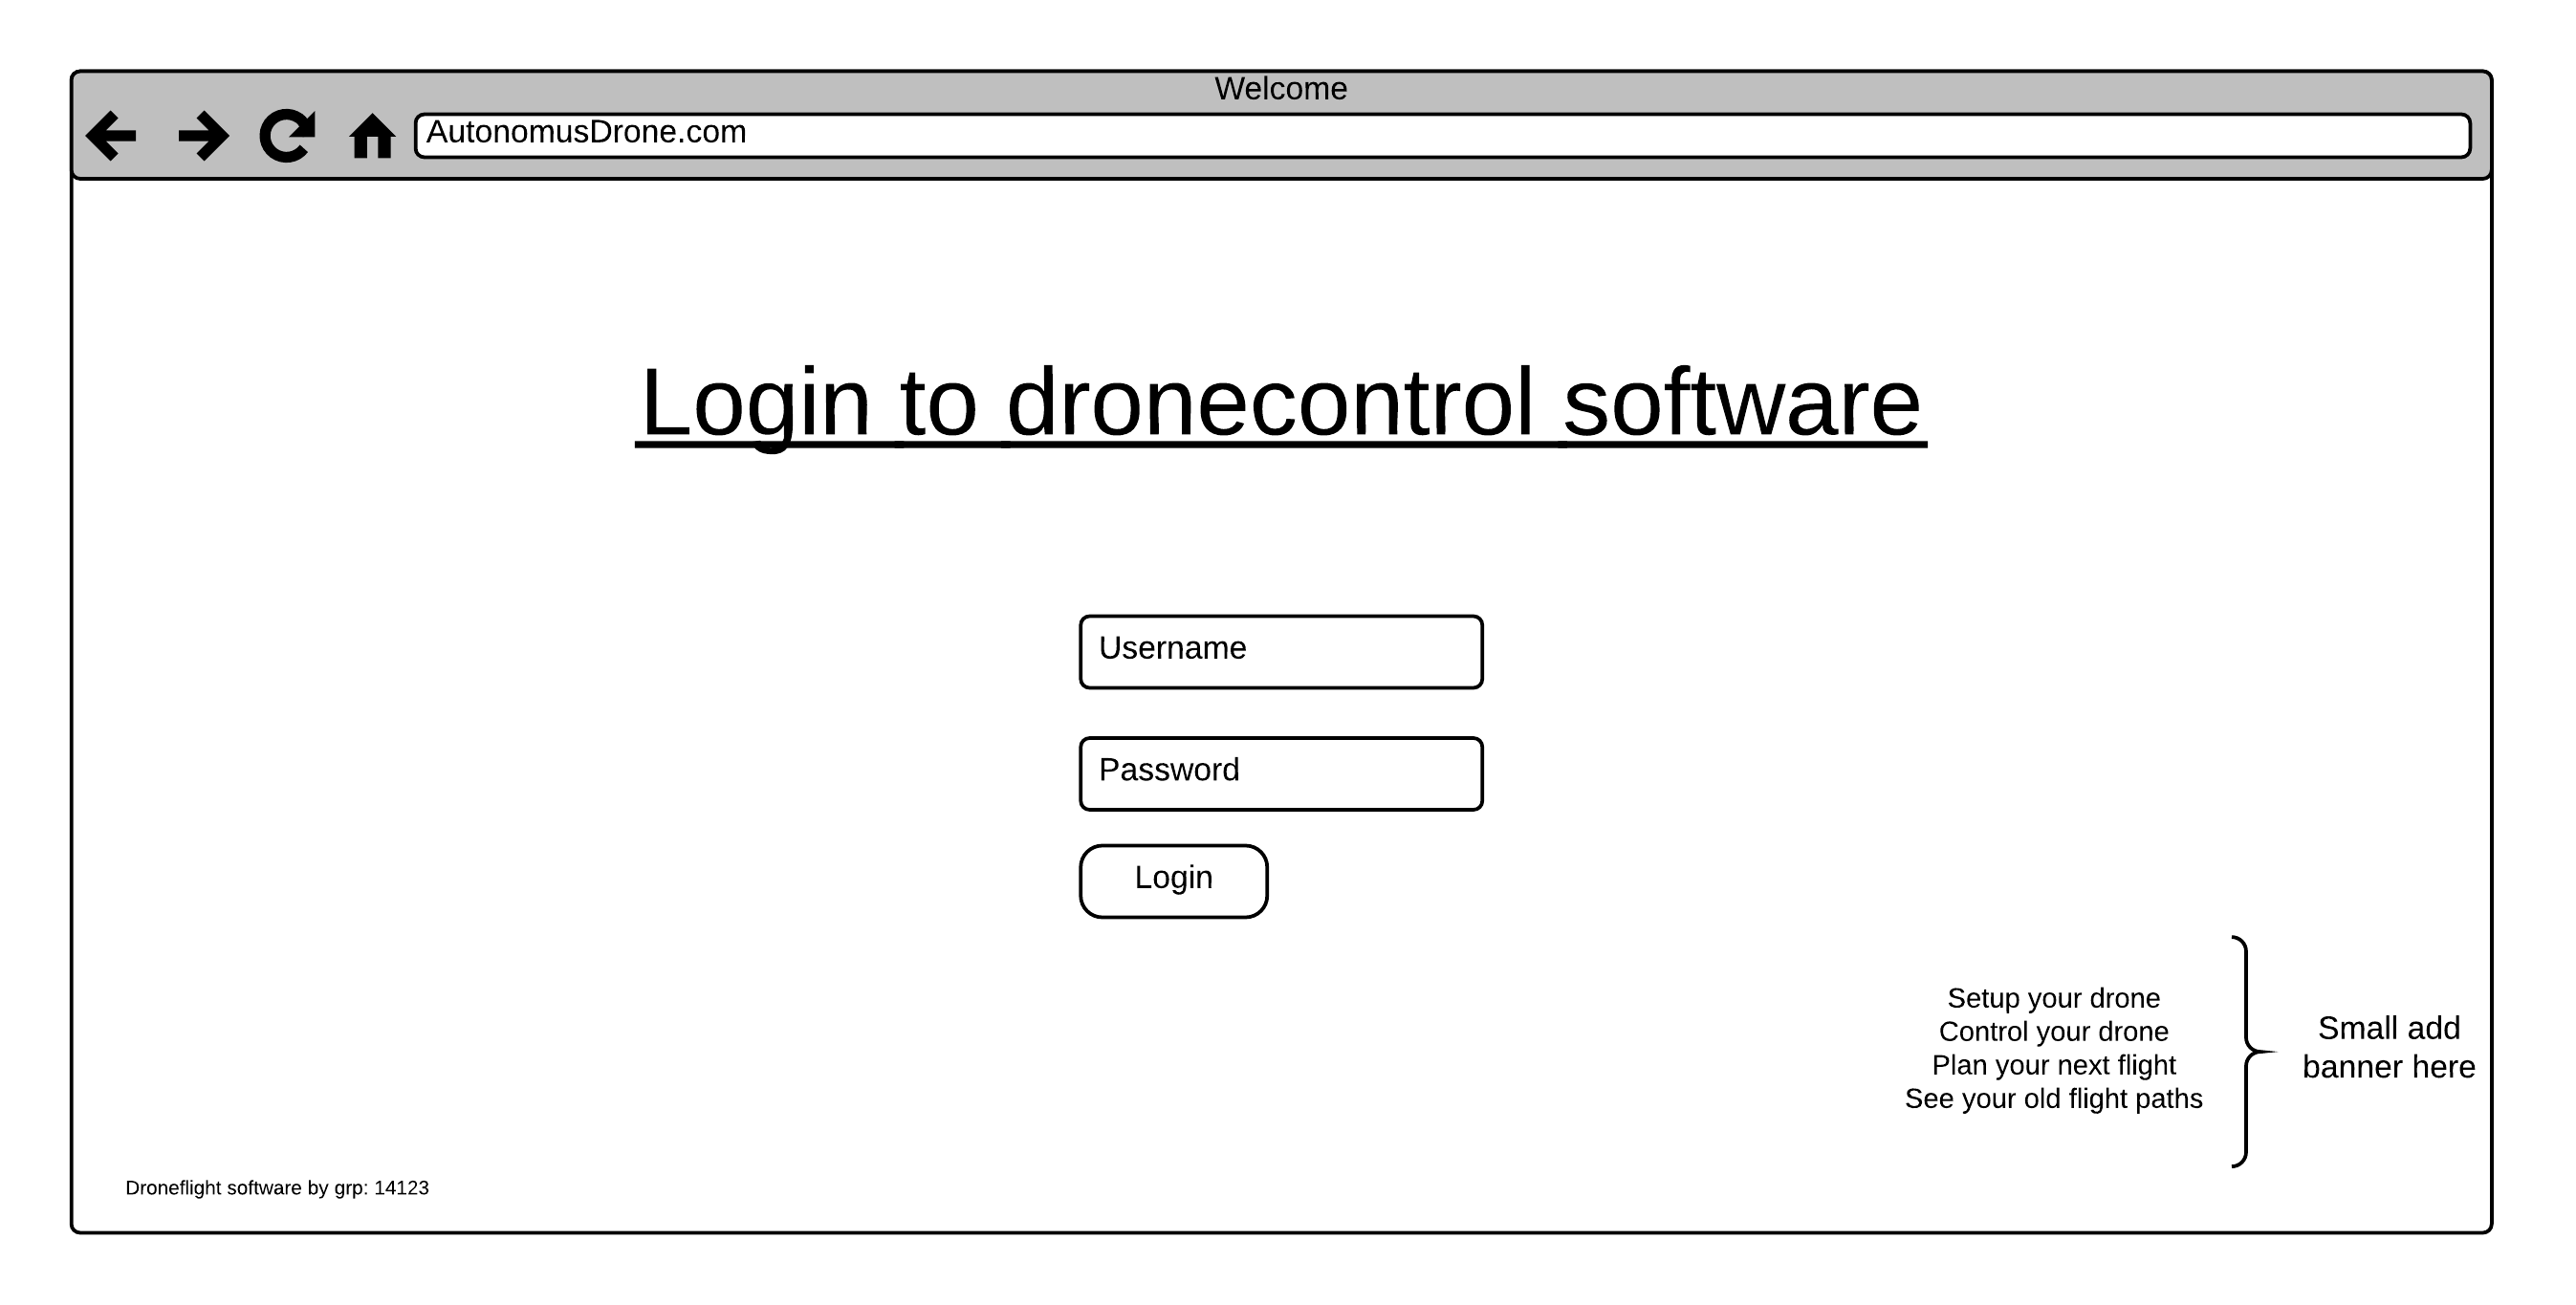
\includegraphics[width=0.7\textwidth]{Billeder/UI_mockups/login.png}
	\vspace{-5pt}
	\caption{Login vindue}
	\label{fig:mockup_login}
\end{figure}

På figuren \ref{fig:mockup_login} ses login vinduet som brugeren bliver præsenteret for når han ønsker at interagere med systemet. Her ville brugeren kunne login og efterfølgende opsætte flyveruter, se gamle ruter og billeder fra forrige flyvninger. \newpage

\vspace{-5pt}
 %Index mockup
 \begin{figure}[H]
 	\centering
 	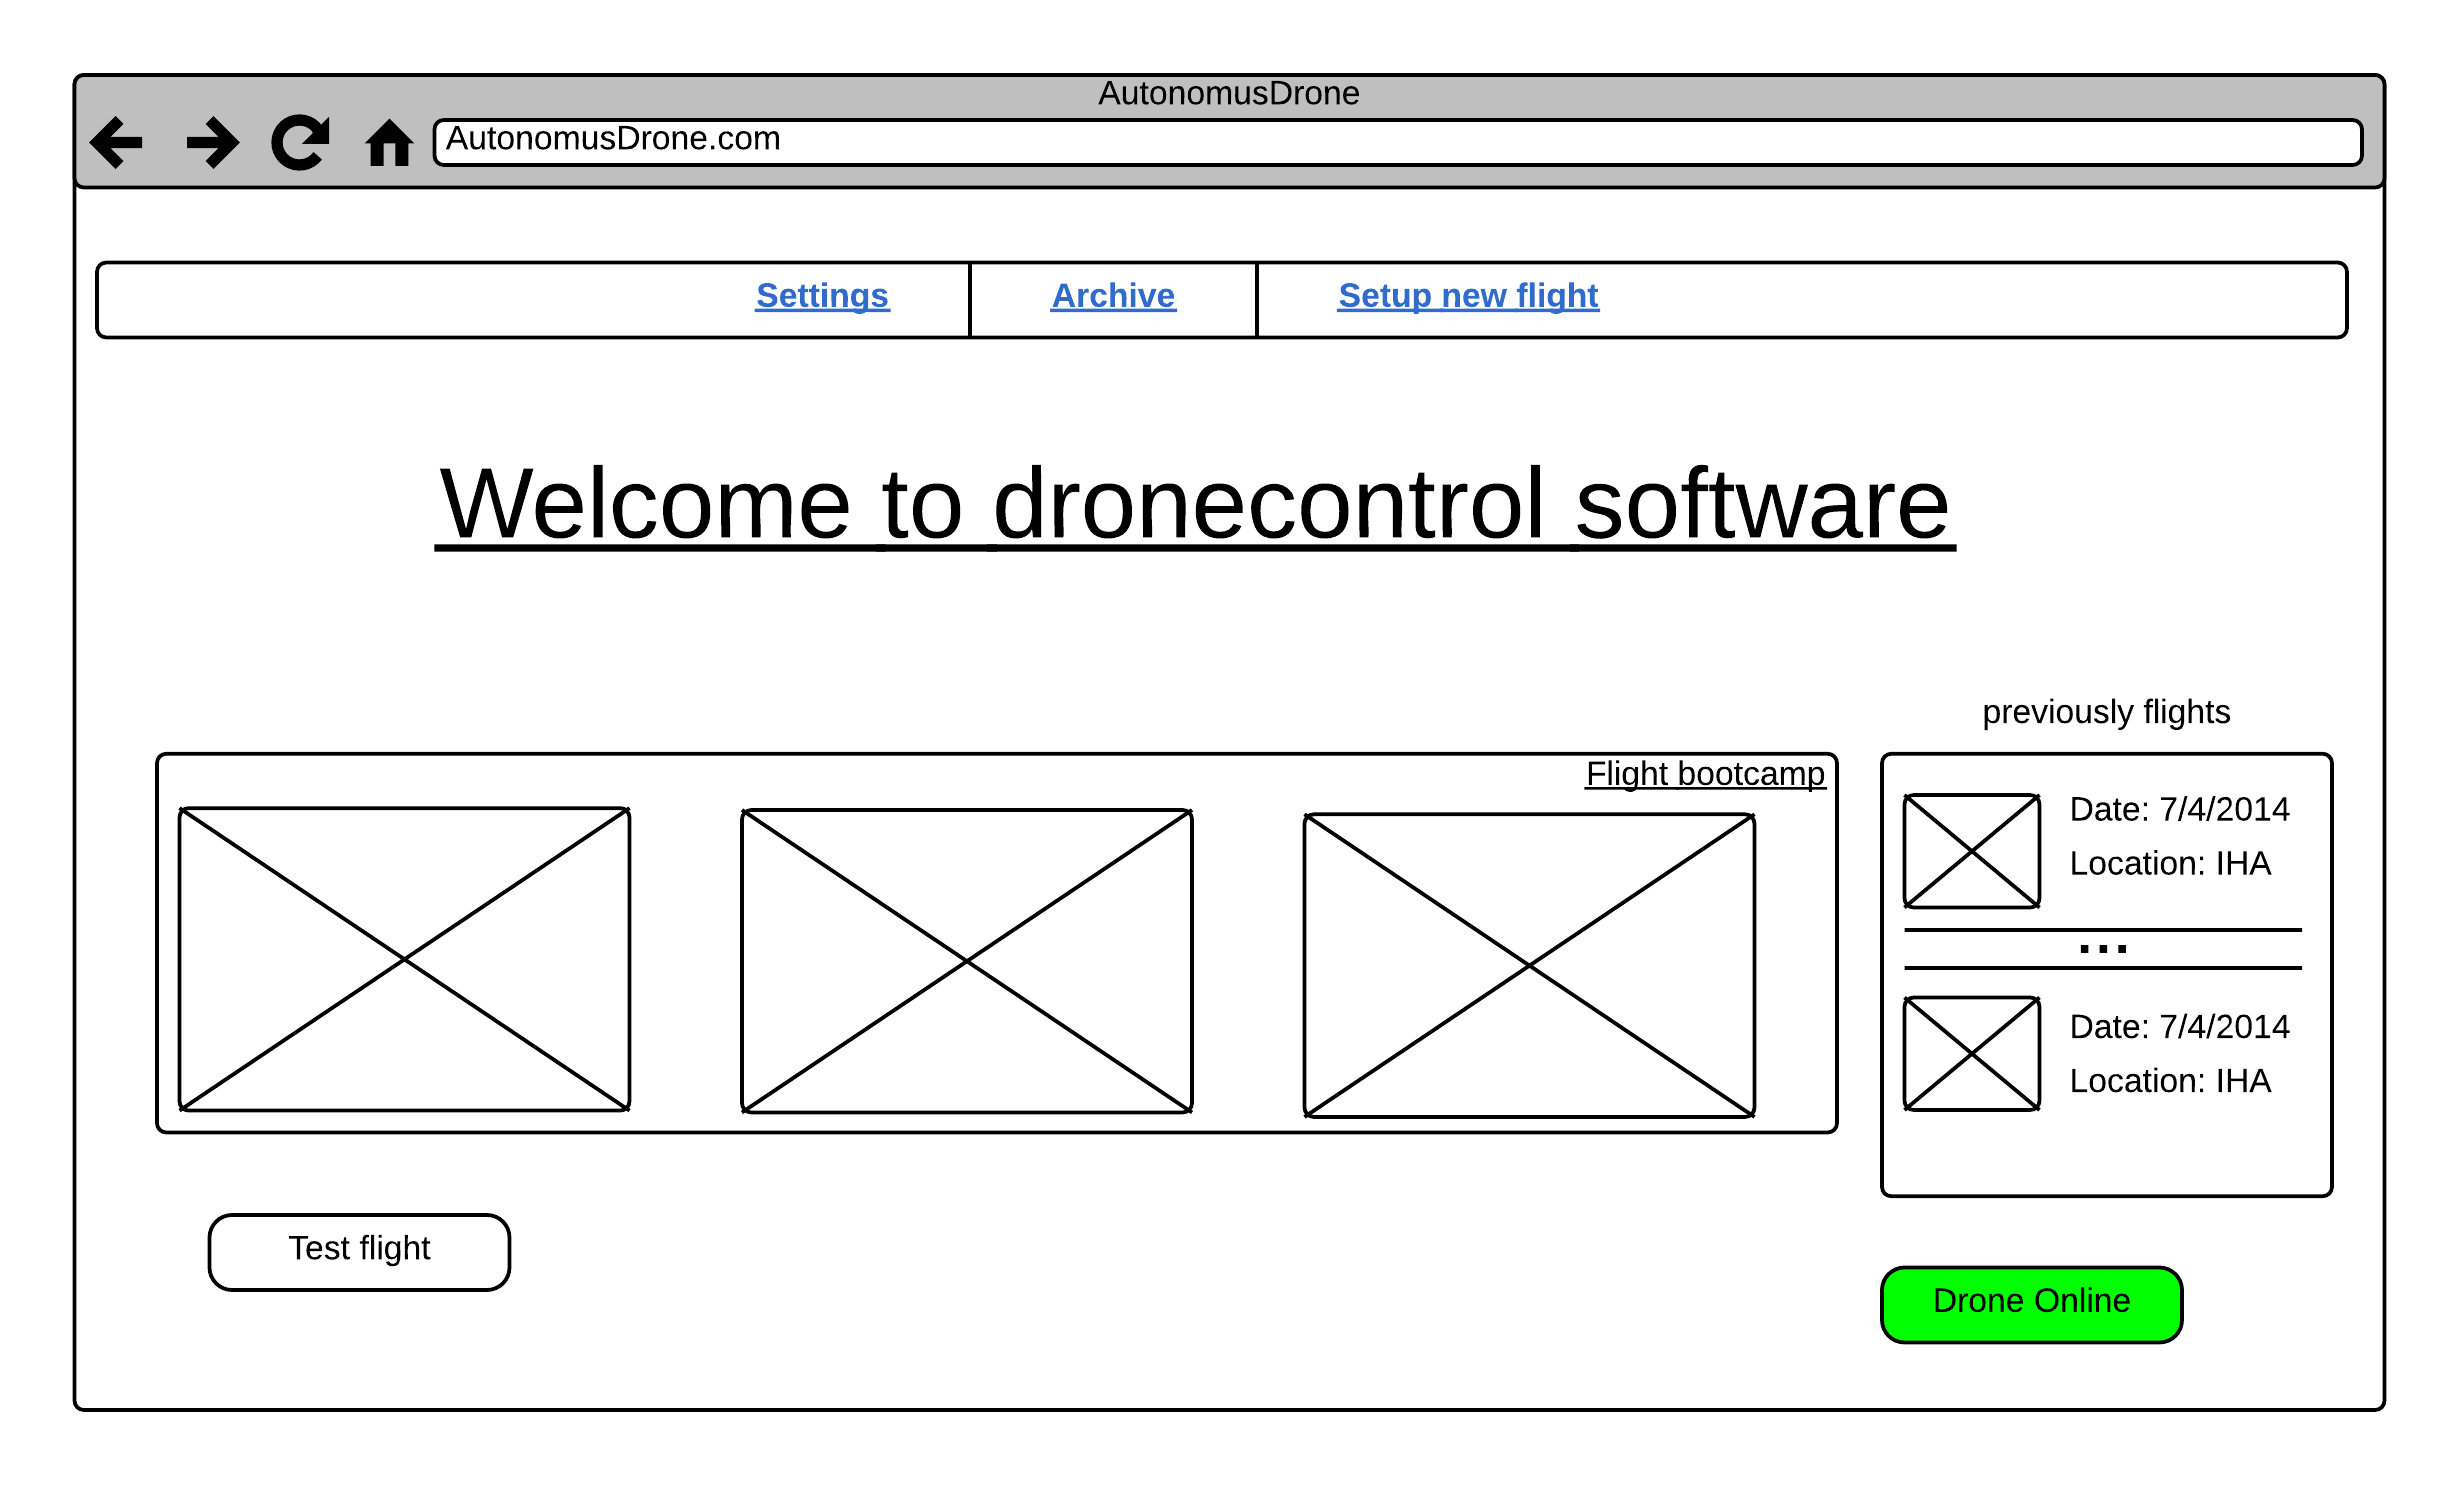
\includegraphics[width=0.7\textwidth]{Billeder/UI_mockups/index.png}
 	\vspace{-5pt}
 	\caption{Velkommen vindue}
 	\label{fig:mockup_welcome}
 \end{figure} 
 
Efter at have logget ind i systemet bliver brugeren præsenteret for velkommen skærmen \ref{fig:mockup_welcome}. Her har brugeren mulighed for at oprette forbindelse til dronen, lave en test flyvning hvilket får dronen til at hoover få sekunder og lande og så lande igen. Menu bjælken "Flight bootcamp" er en quick-guide til systemet, bjælken kan lukkes ned hvis brugeren ikke ønsker at bruge quick-guiden. På forsiden kan brugeren også se en liste med et uddrag de sidste flyvninger. Øverst på siden har brugeren mulighed for at navigere til indstillinger for dronen, den fulde liste af tidligere flyvninger og opsætte nyflyvning. \newpage

\vspace{-5pt}
%Settings mockup
\begin{figure}[H]
	\centering
	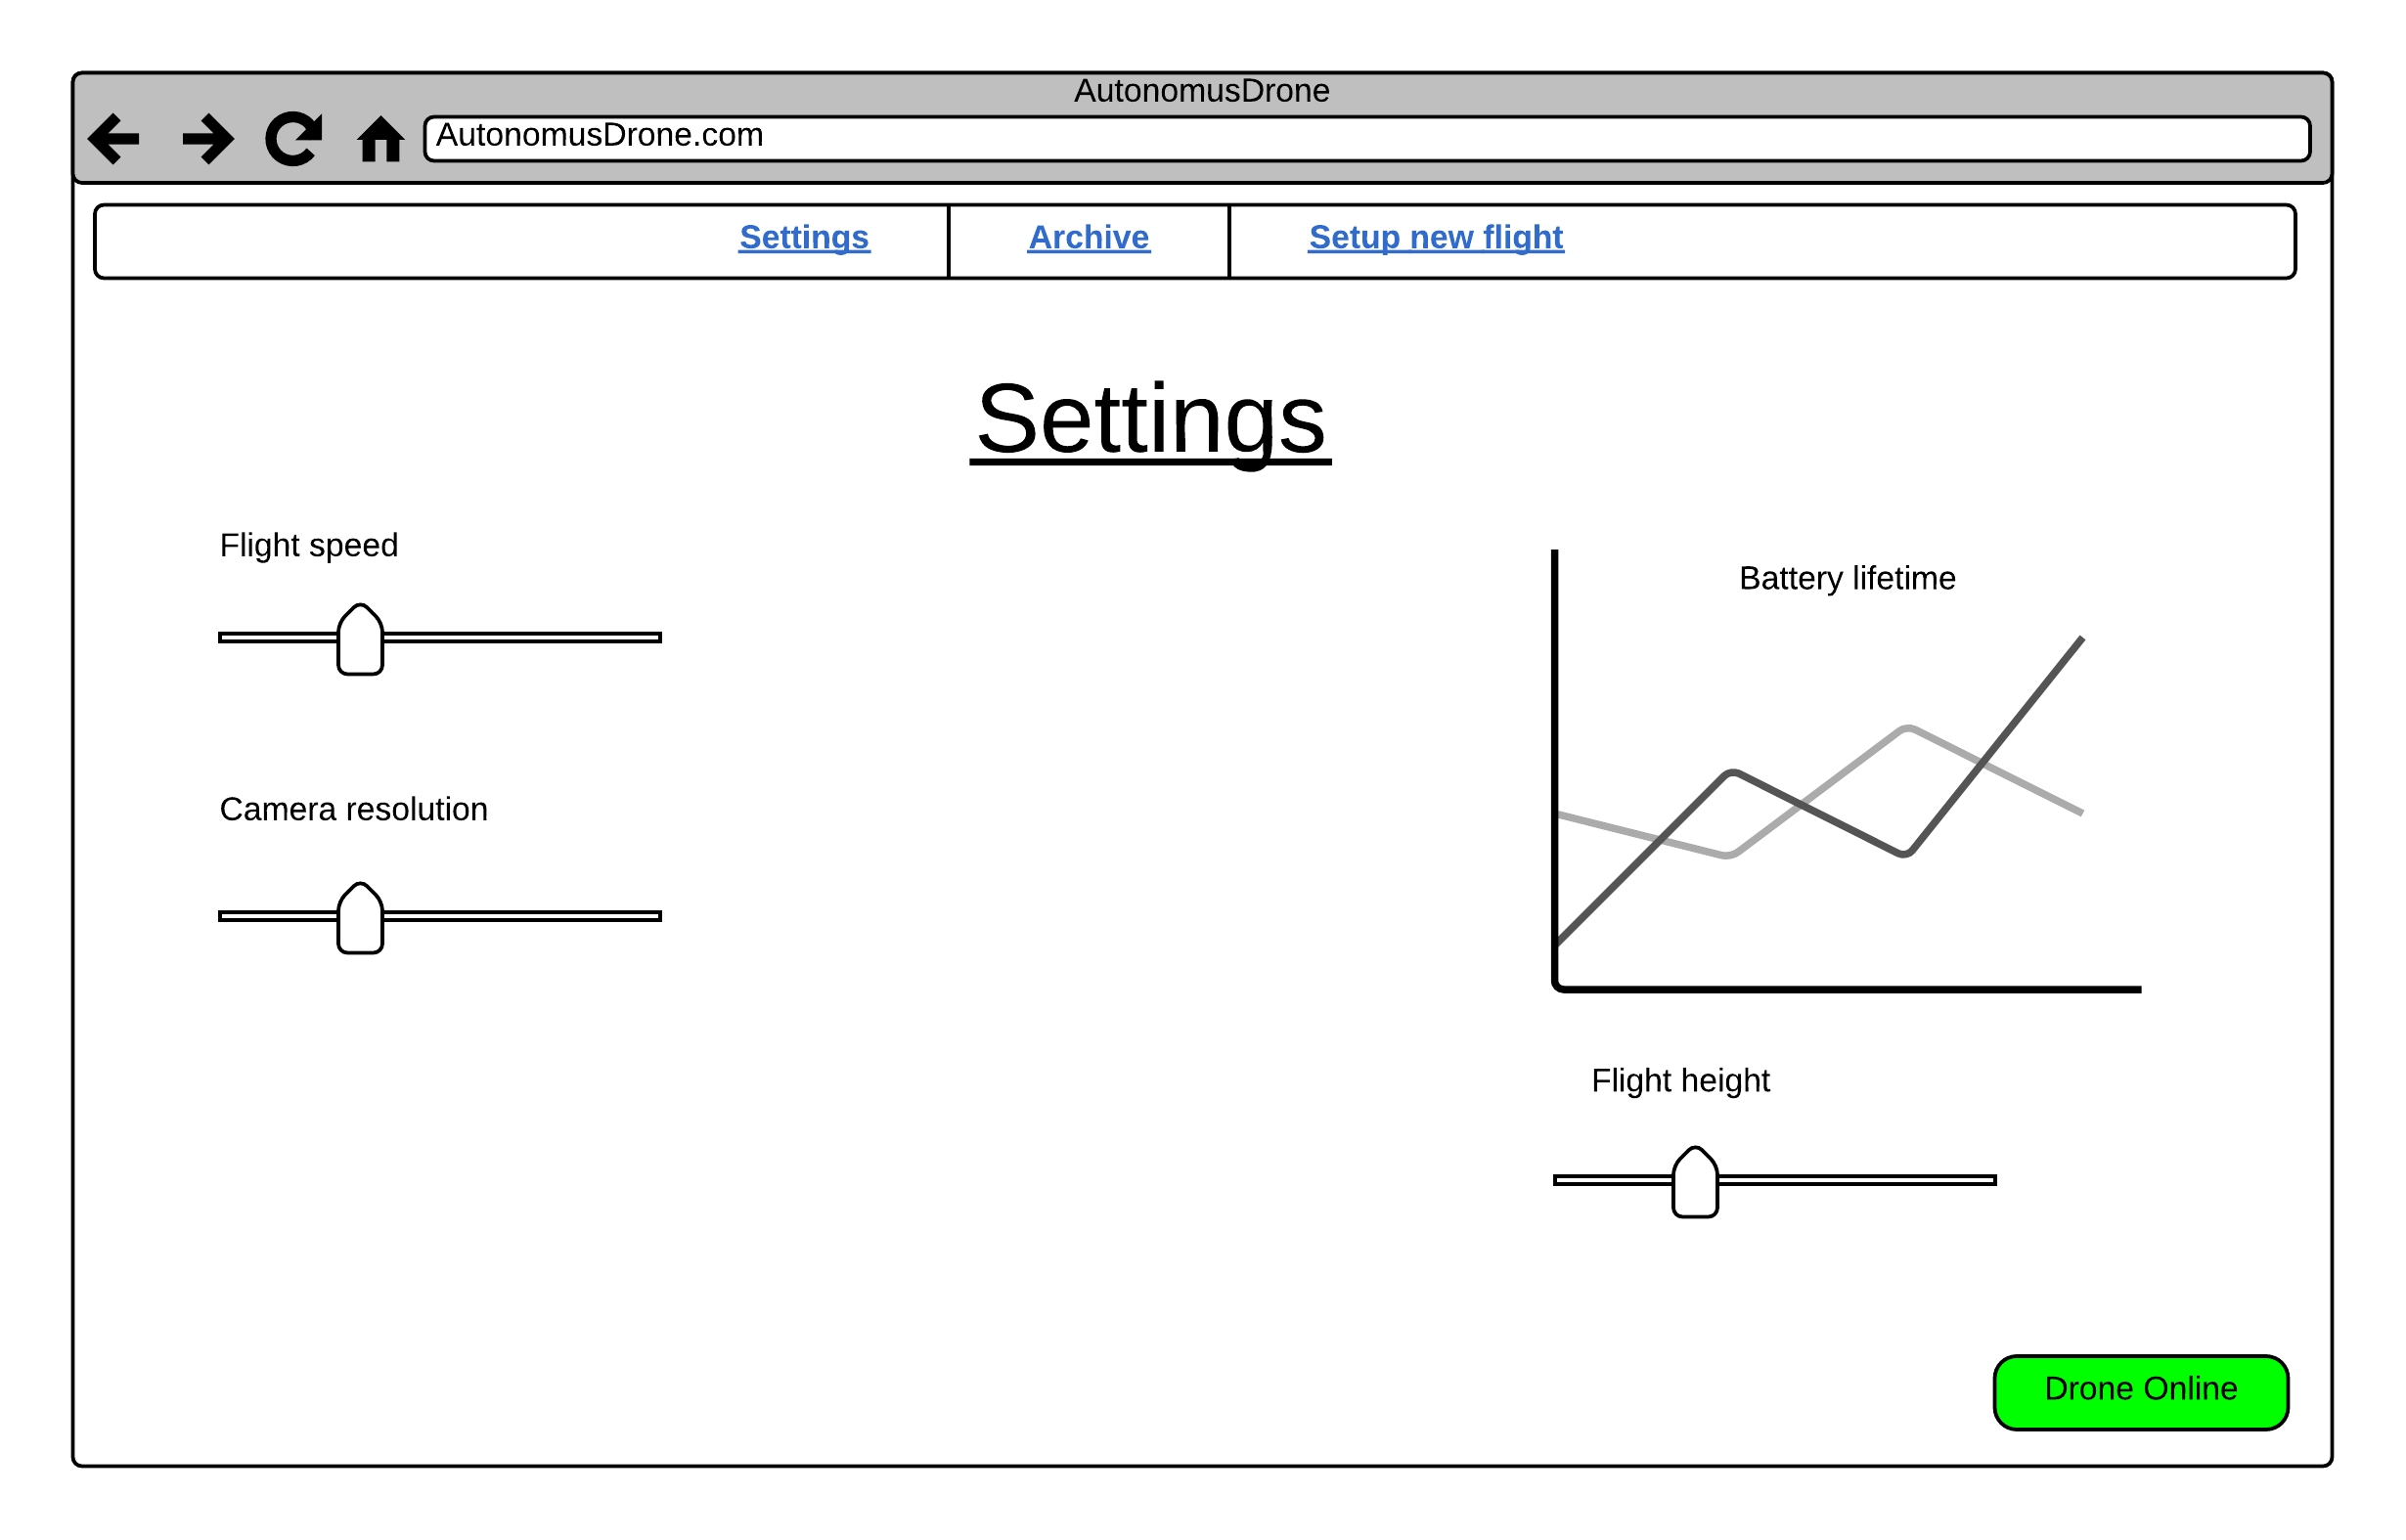
\includegraphics[width=0.7\textwidth]{Billeder/UI_mockups/settings.png}
	\vspace{-5pt}
	\caption{Indstillinger vindue}
	\label{fig:mockup_settings}
\end{figure}

Settings vinduet giver brugeren mulighed for at lave generelle opsætninger som ænder dronens og webapplikationens adfærd. Brugeren kan også få et overblik over dronens batteriforbrug via en graf.

\vspace{-5pt}
%Archive mockup
\begin{figure}[H]
	\centering
	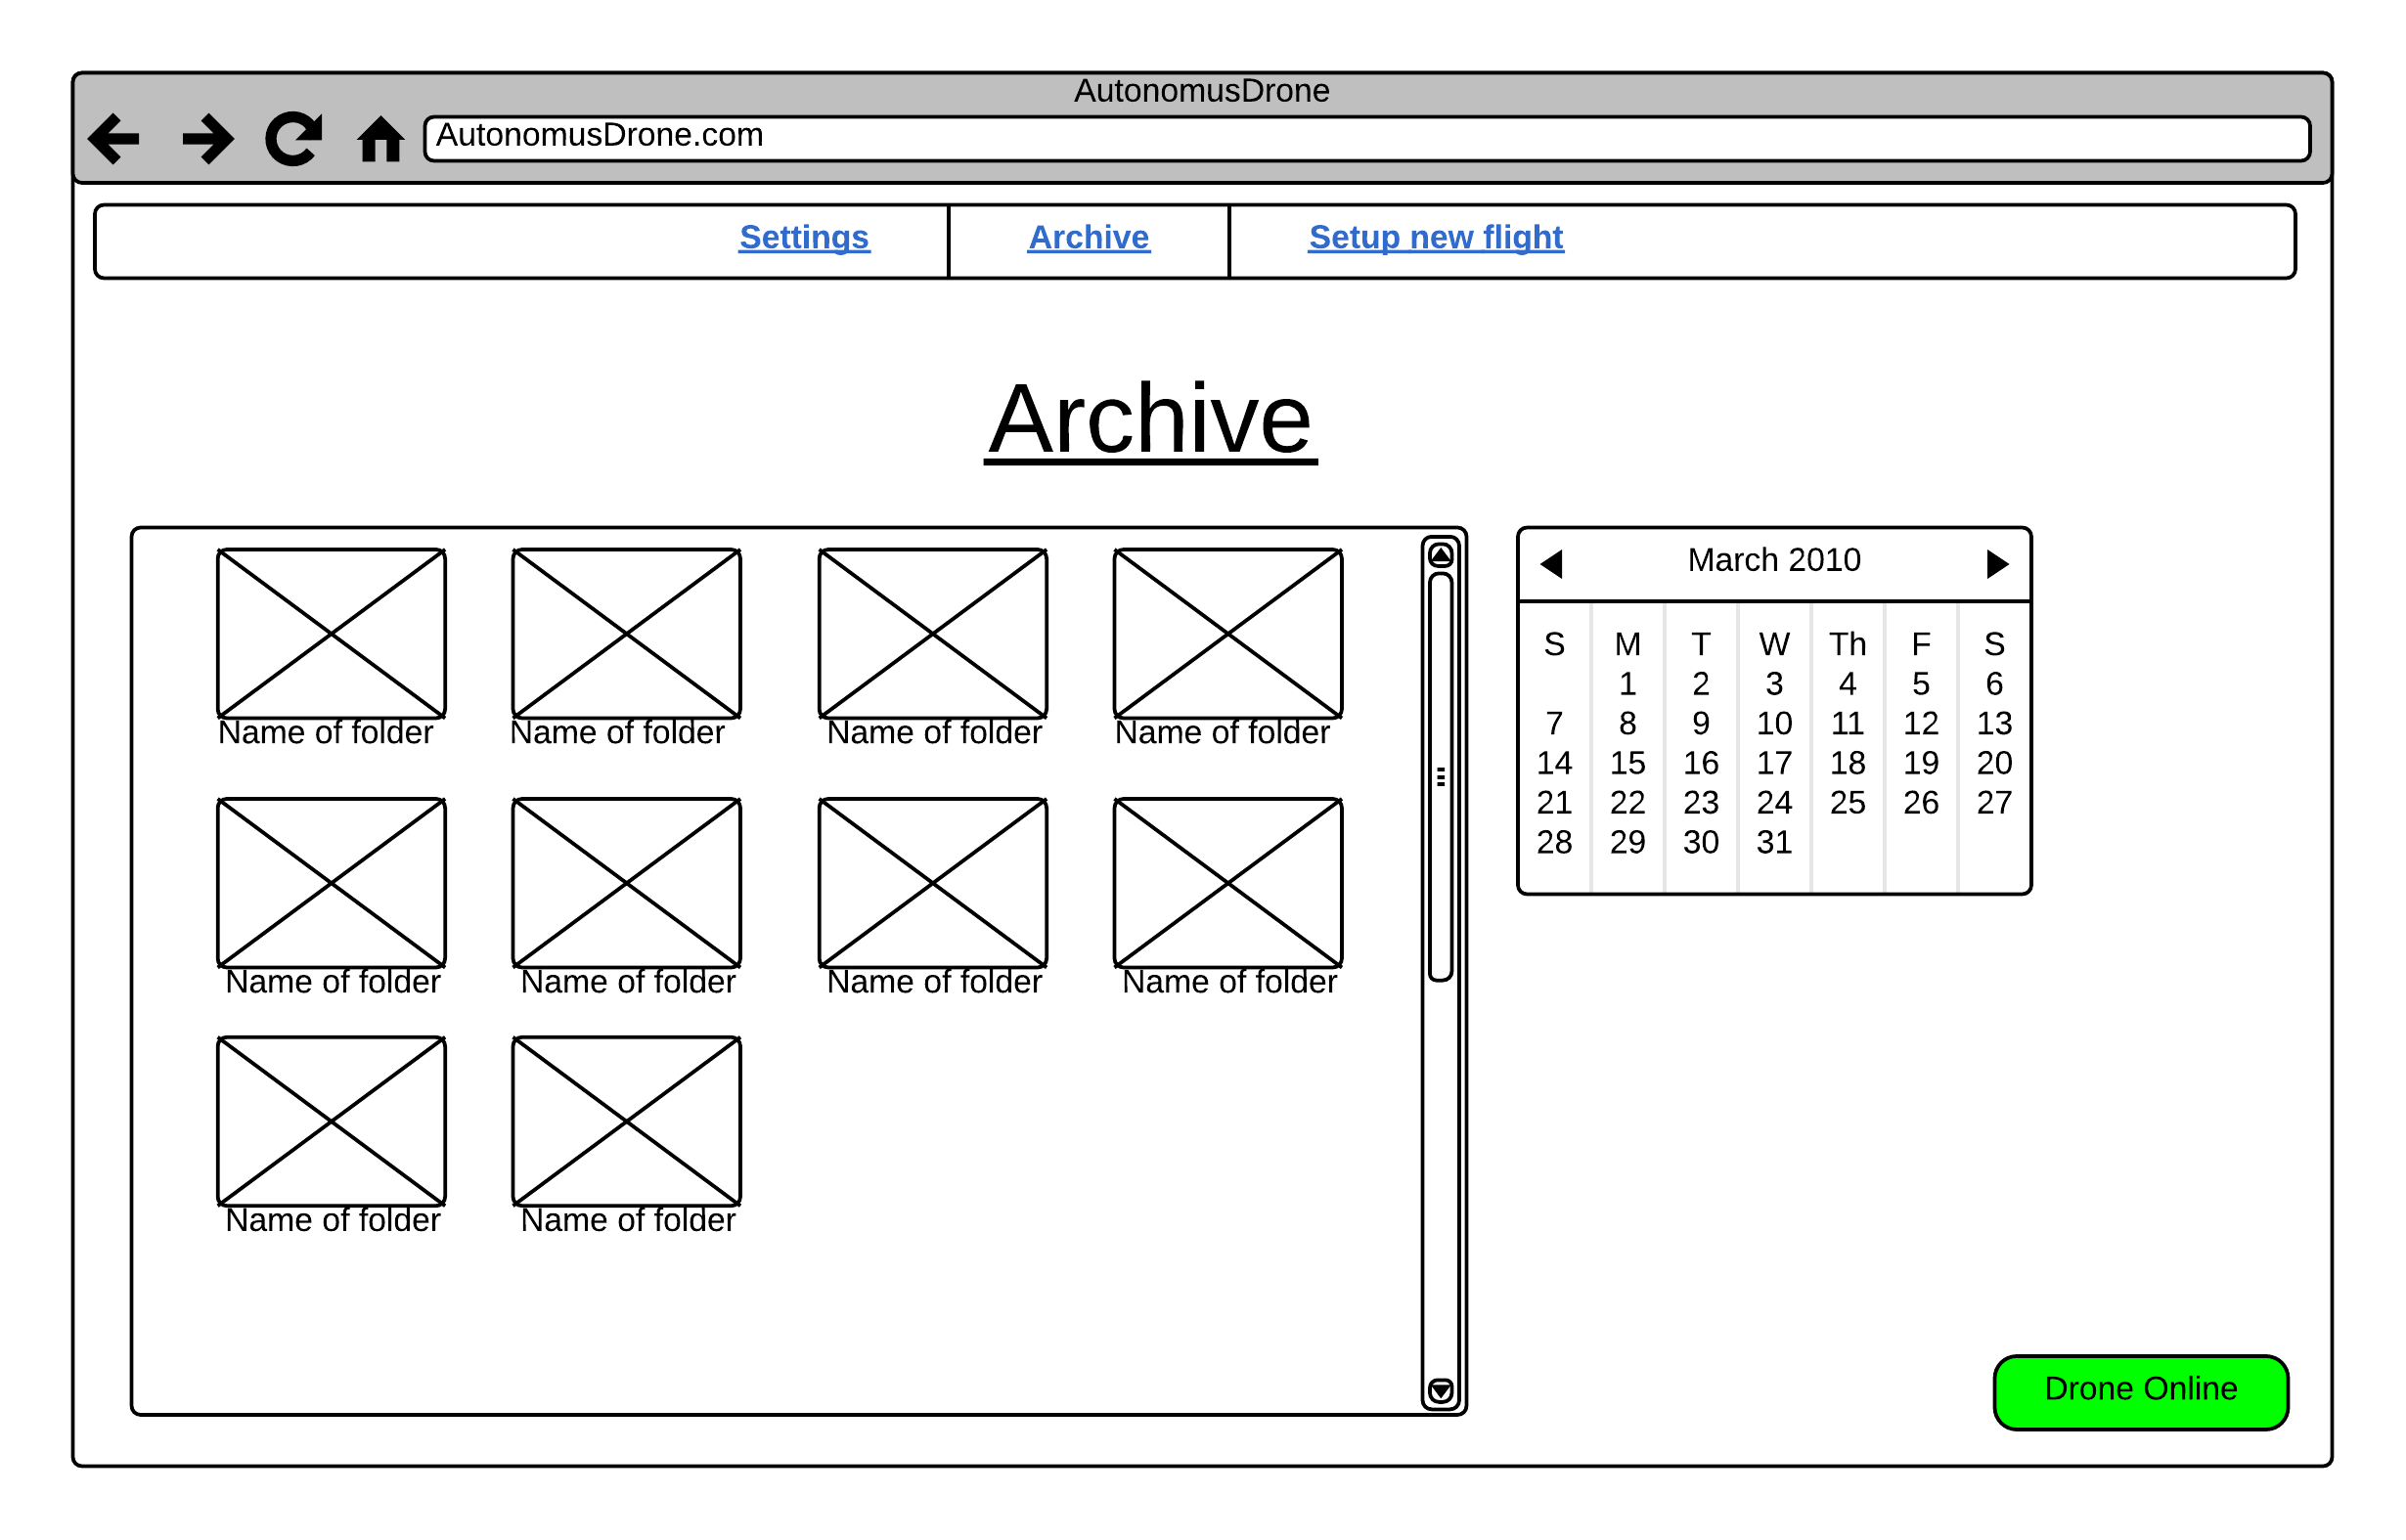
\includegraphics[width=0.7\textwidth]{Billeder/UI_mockups/archive.png}
	\vspace{-5pt}
	\caption{Historik vindue}
	\label{fig:mockup_archive}
\end{figure}

I archive menuen har brugeren mulighed for at se alle sine tidligere flyvninger som bliver præsenteret med en mappestruktur. Kalenderen kan bruges til at hurtigt finde frem til en bestem periode i historikken. Ved double klik på en tidligere flyvning åbnes mappen.

\vspace{-5pt}
%Archive choosen mockup
\begin{figure}[H]
	\centering
	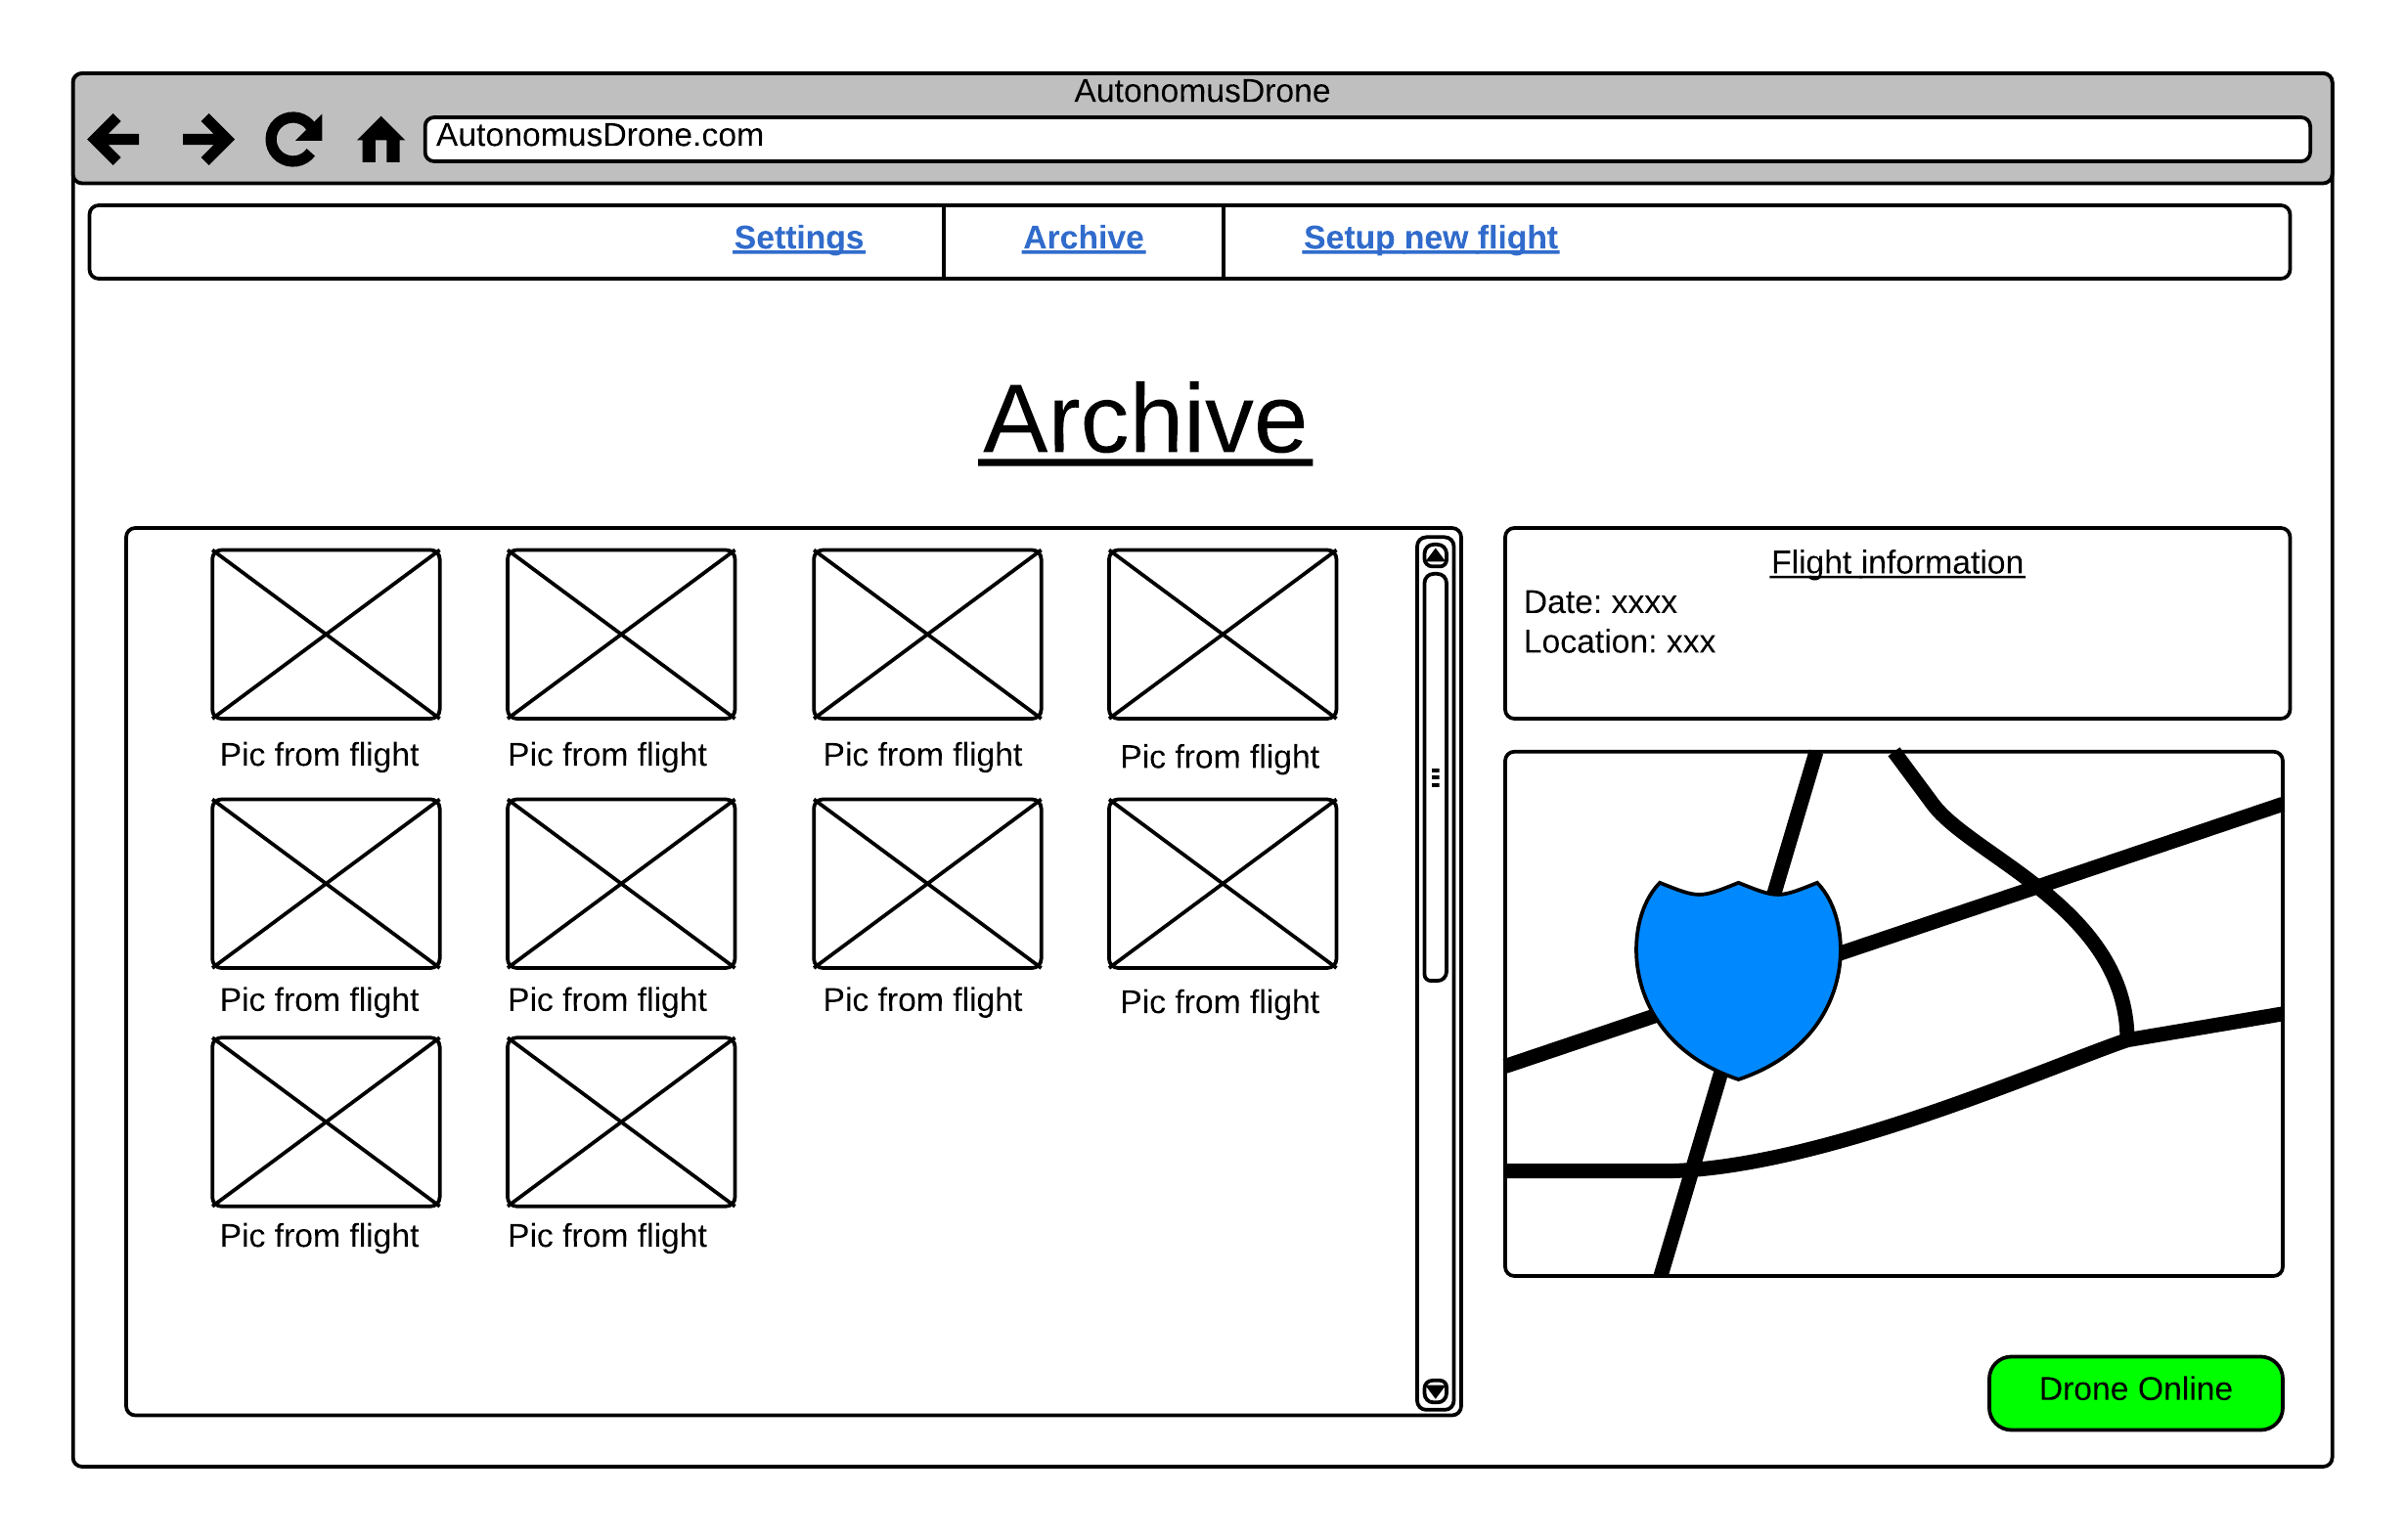
\includegraphics[width=0.7\textwidth]{Billeder/UI_mockups/archive_choosen.png}
	\vspace{-5pt}
	\caption{Tidligere flyverute valgt}
	\label{fig:mockup_archive_choosen}
\end{figure}

Når en tidligere flyvning er valgt, bliver brugeren præsenteret for information omkring den på gældende rute samt billederne taget på ruten. Et kort viser hvilken rute dronen fløj under flyvningen.

\vspace{-5pt}
%Setup new flight mockup
\begin{figure}[H]
	\centering
	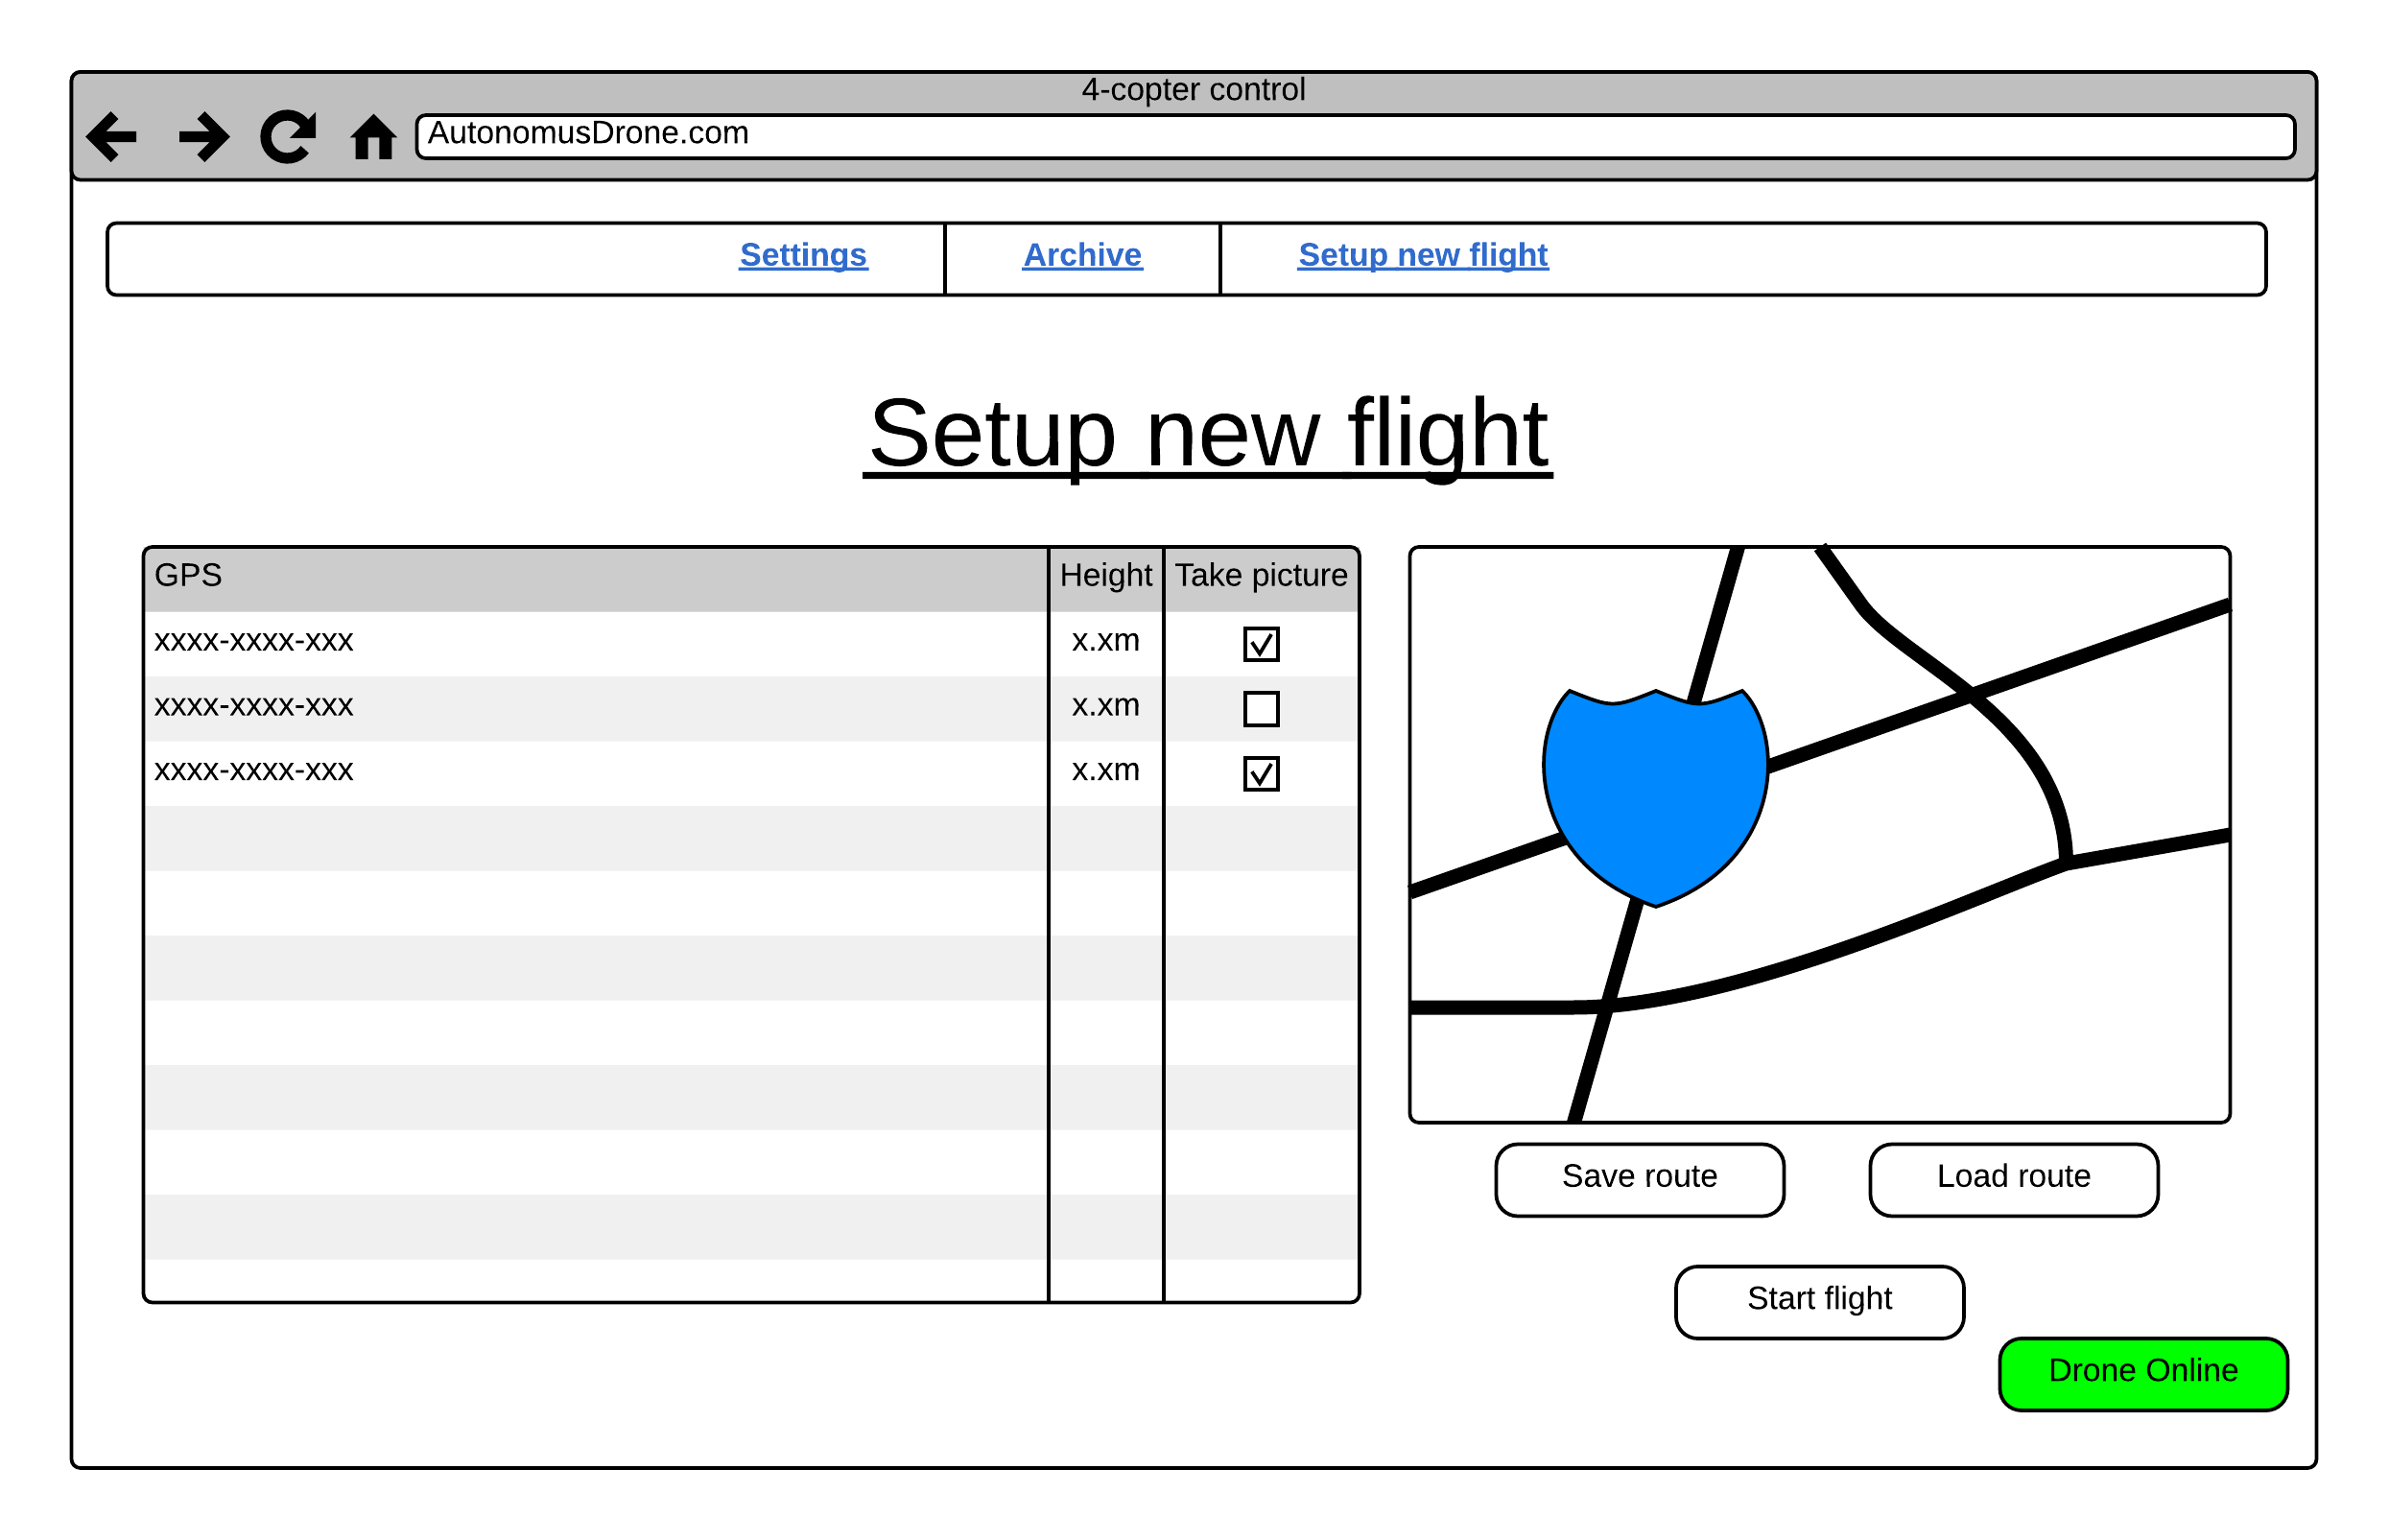
\includegraphics[width=0.7\textwidth]{Billeder/UI_mockups/setup_new_flight.png}
	\vspace{-5pt}
	\caption{Ny flyverute}
	\label{fig:mockup_setup_new_flight}
\end{figure}

I Setup new flight menuen kan brugen planlægge en ny flyverute. Ved at klikke på kortet og derved lave waypoints kan brugeren tegne den ønskede flyverute. Div. waypoints bliver så præsenteret som GPS lokationer i tabellen til venstre for kortet. I tabellen kan brugeren også bestemme hvilke højde dronen skal befinde sig i på det givet koordinat, brugeren kan også bestemme om dronen skal tage et billede på lokationen. Brugeren har mulighed for at gemme den ny konstrueret rute og hente den til senere brug. 